\section{Preliminary Results from Belle Open Data}

Figure~\ref{fig:multPID} shows the multiplicity distribution of identified particles (pions, kaons and proton) obtained after 
applying the selection on the particle transverse momentum (0.1 $<p_{\rm T}<$ 4.0 GeV/$c$). 
The dominant contribution to the total multiplicity is coming as expected from pions.
In Fig.~\ref{fig:multHadron}, the charged hadron multiplicity distribution $N$ is shown: the largest raw particle multiplicity observed in these events is about 70 before corrections for tracking efficiency, fakes and multiple reconstruction rate. 

\begin{figure}[!htb]
\begin{center}
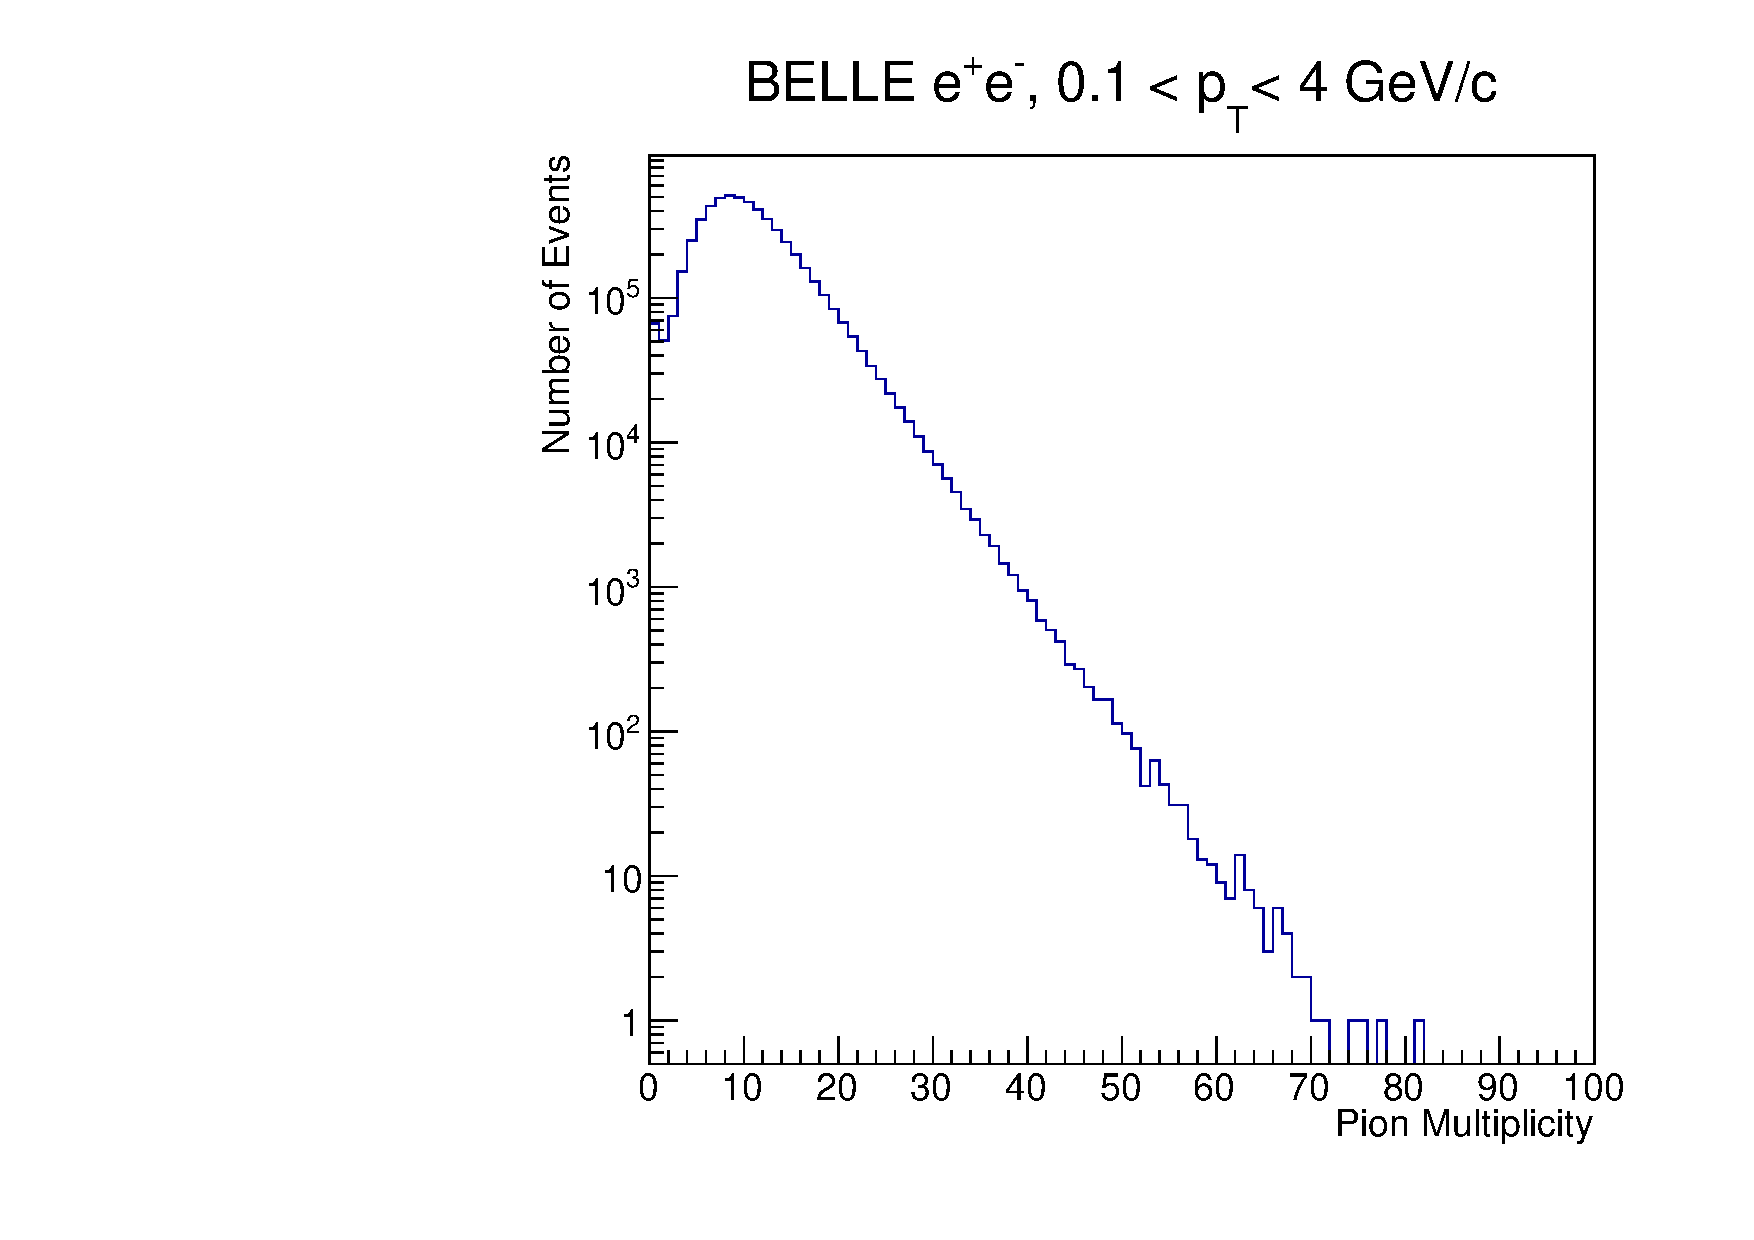
\includegraphics[width=.32\textwidth]{figures/pion_mult.pdf}
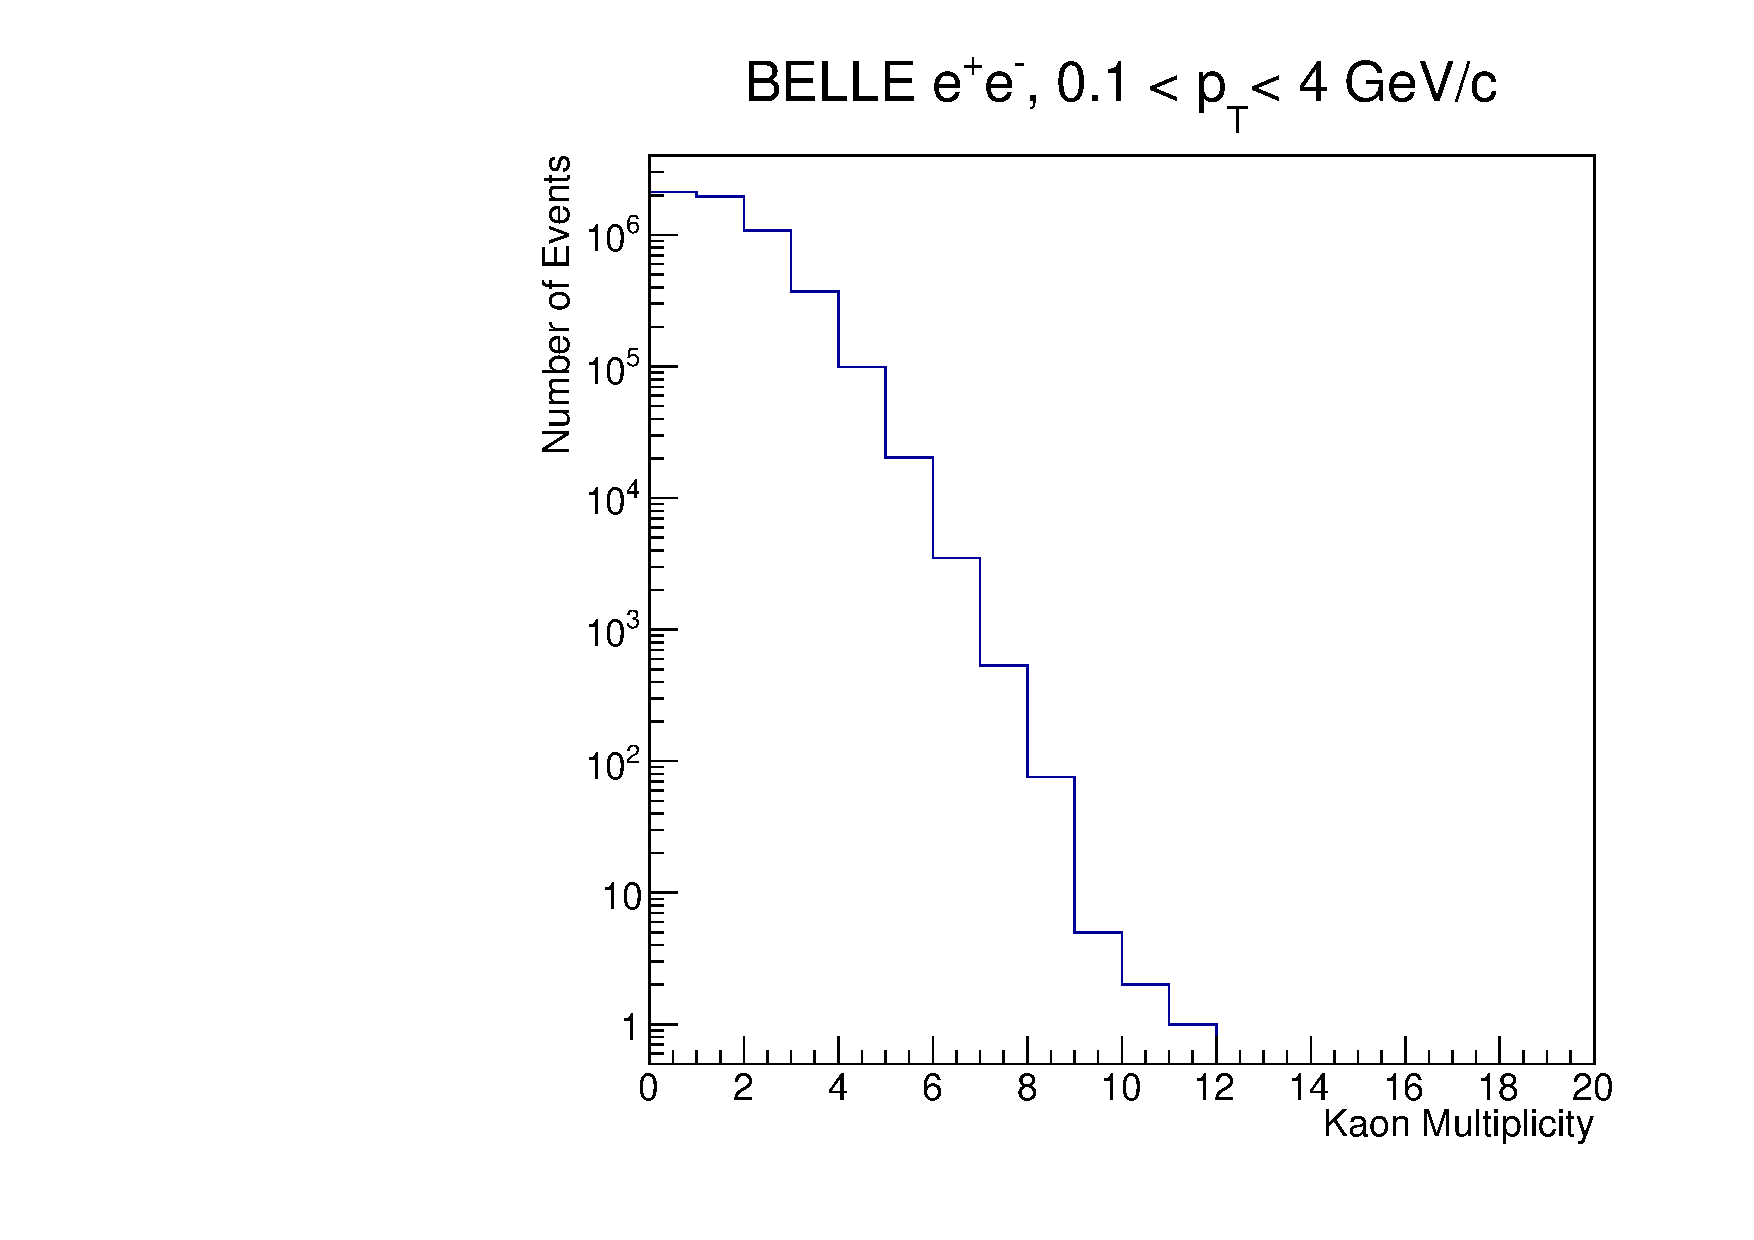
\includegraphics[width=.32\textwidth]{figures/kaon_mult.pdf}
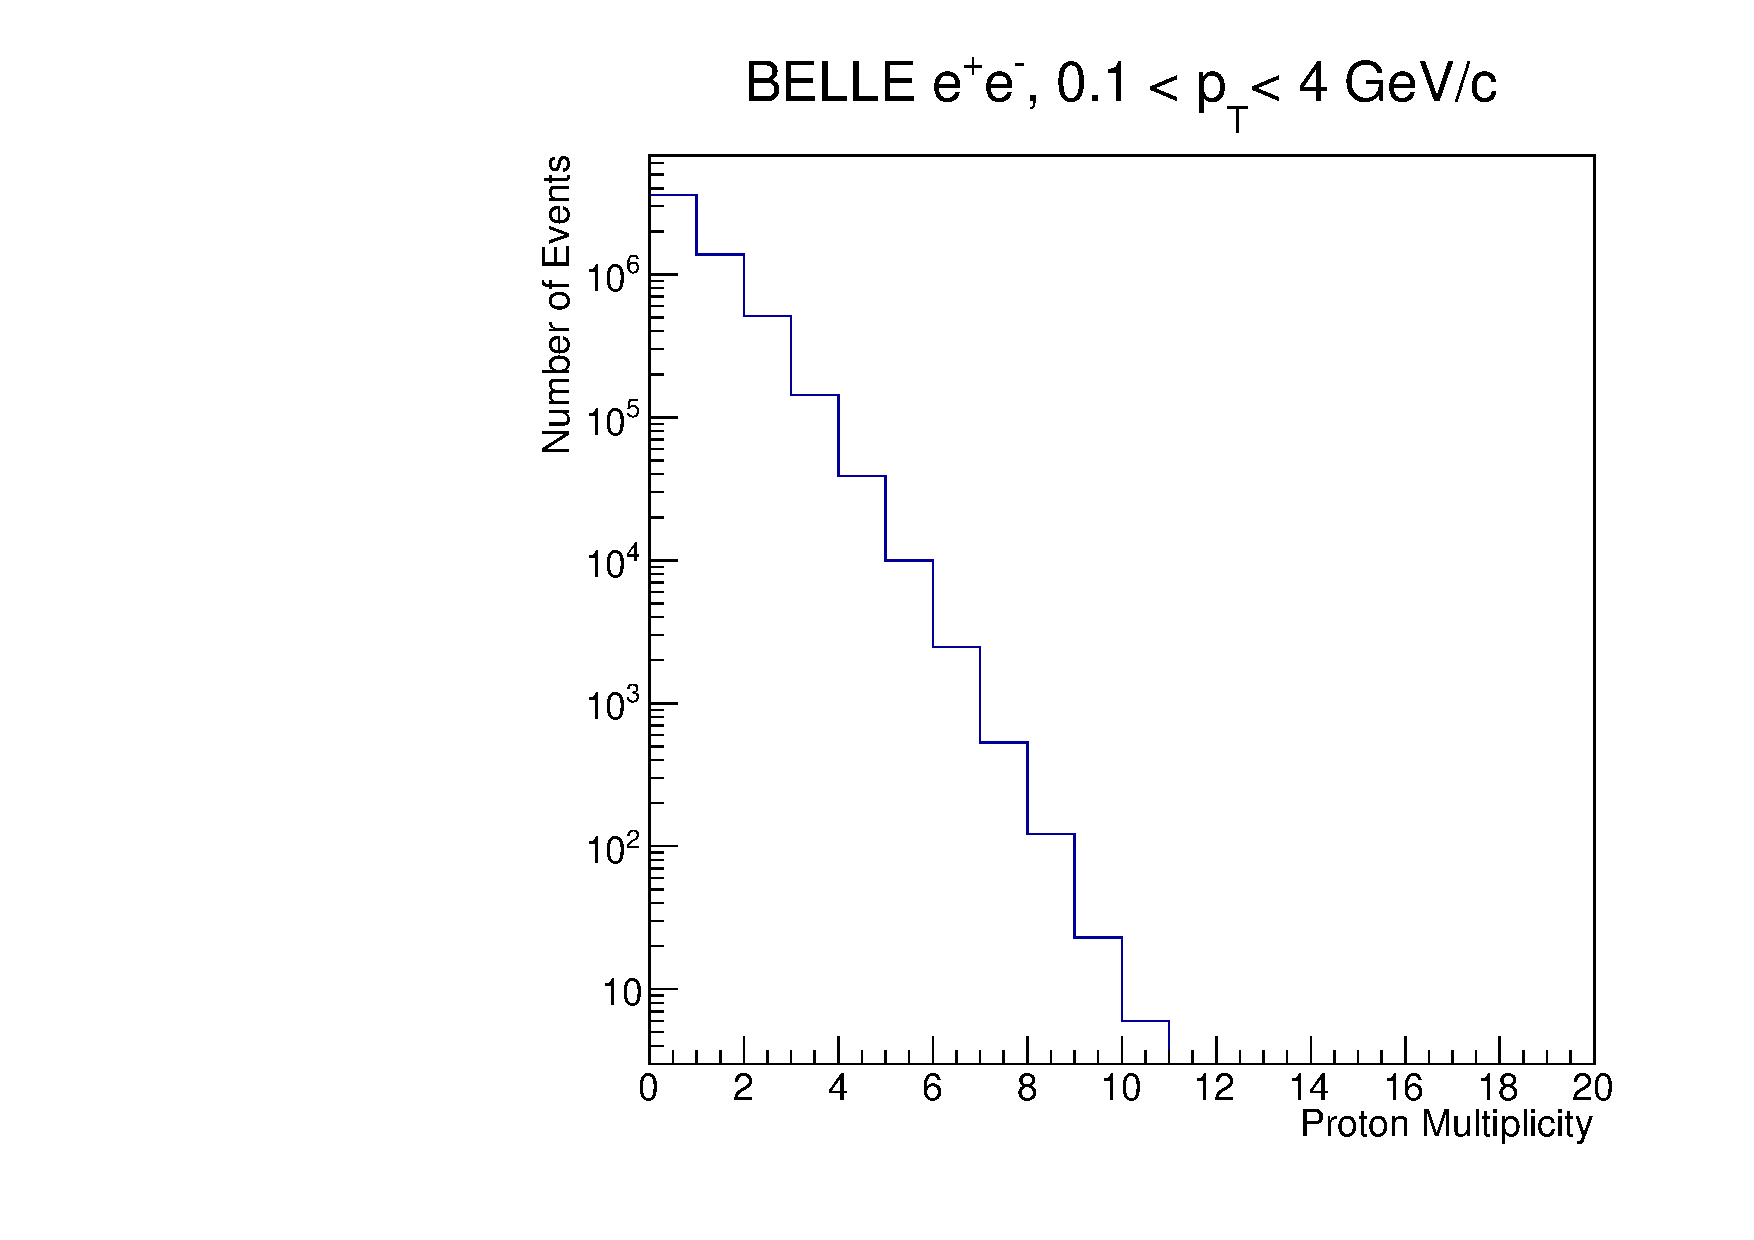
\includegraphics[width=.32\textwidth]{figures/proton_mult.pdf}
\caption{Uncorrected multiplicity distributions of pions (left), kaons (middle), protons (right) for  particles in the range  0.1 $<p_{\rm T}<$ 4.0 GeV/$c$ in $e^{+}e^{-}$ collisions. }
\label{fig:multPID} 
\end{center}
\end{figure}

\begin{figure}[!htb]
\begin{center}
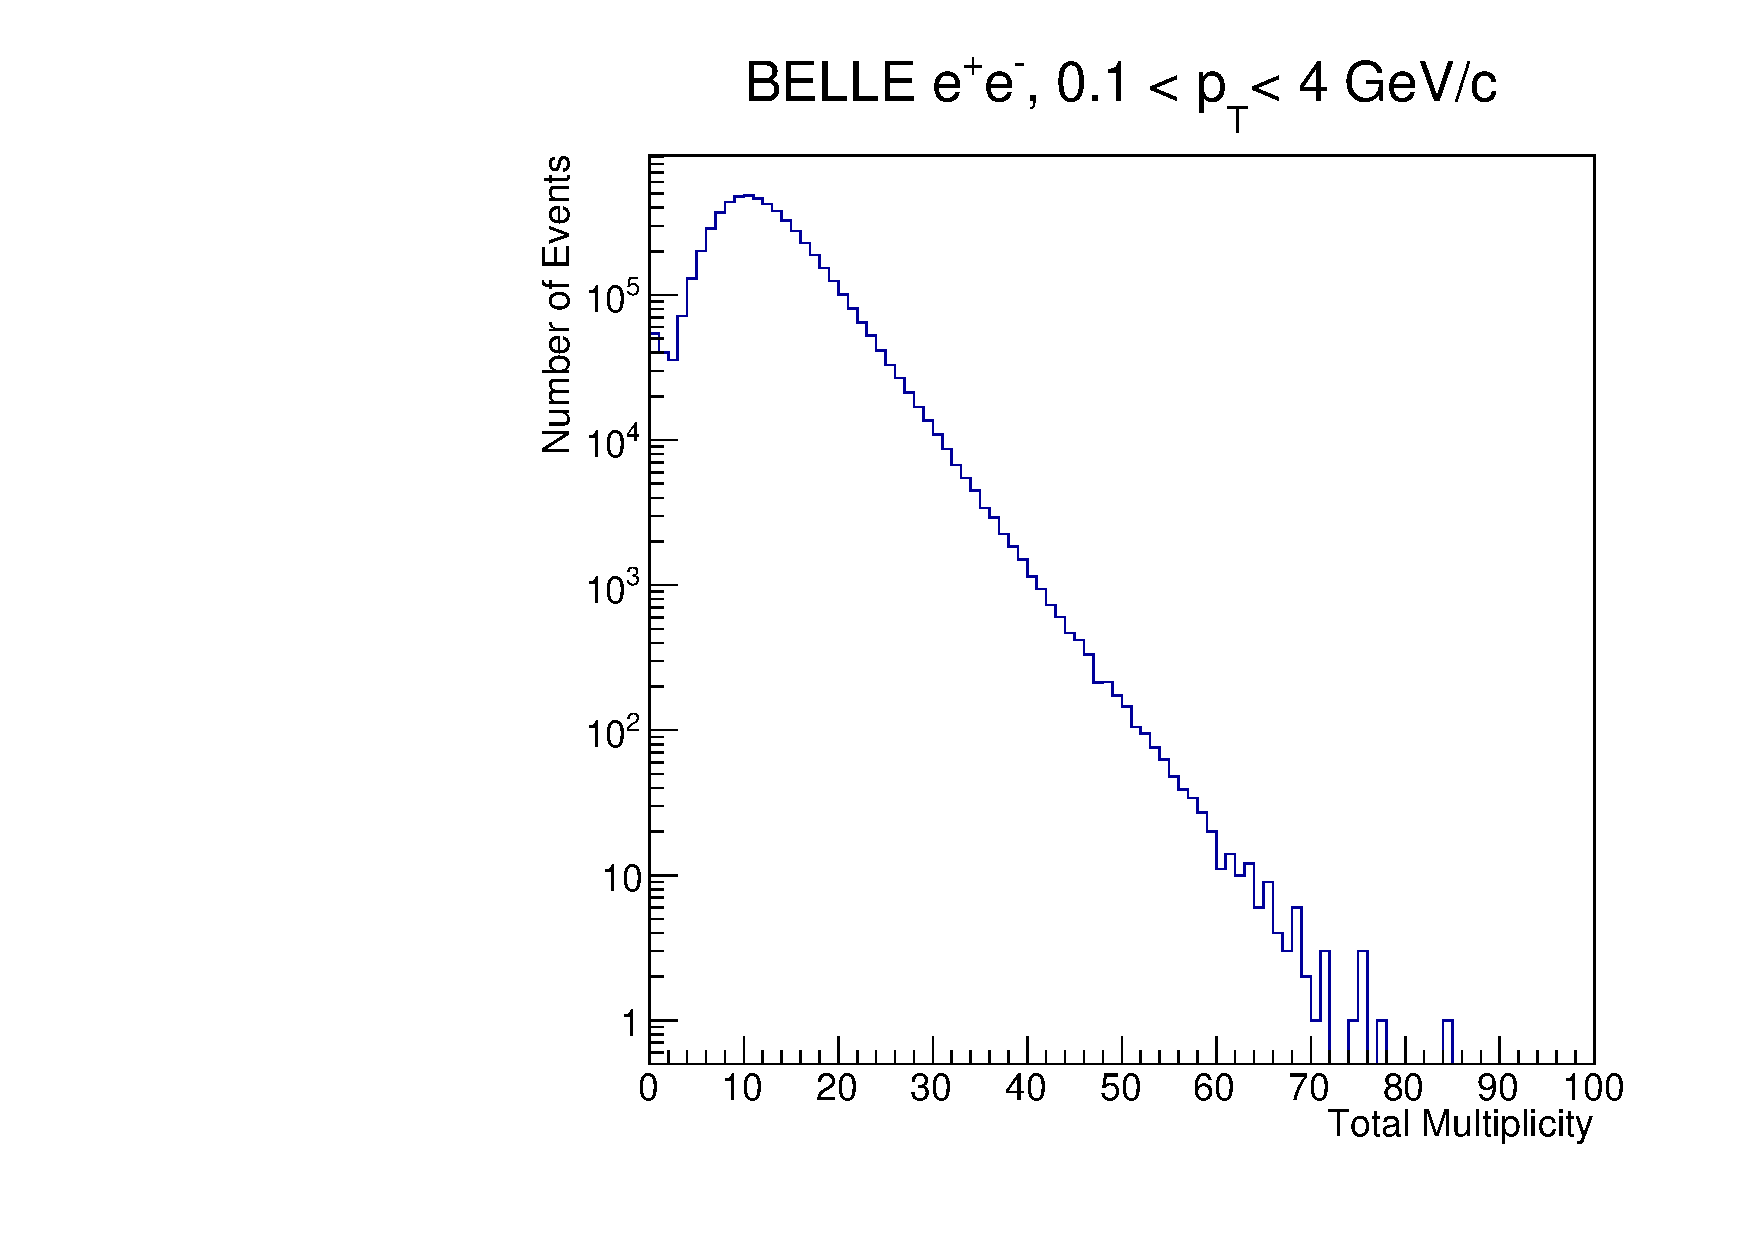
\includegraphics[width=.45\textwidth]{figures/total_mult.pdf}
\caption{Multiplicity distribution of charged hadrons (protons, kaons and pions) for  particles in the range  0.1 $<p_{\rm T}<$ 4.0 GeV/$c$ in $e^{+}e^{-}$ collisions. }
\label{fig:multHadron} 
\end{center}
\end{figure}

In this proposal we present the first study of two particle correlations with $e^{+}e^{-}$ with the Belle experiment using open data.
In Fig.~\ref{fig:ridgeBelle} we compare the two-particle correlation functions for events with low (N$>$20) and high multiplicity(N$>40$). 
In the low-multiplicity result, the dominant features are the correlation peak near $(\Delta\eta,\Delta\phi)=(0,0)$ for pairs of particles originating from the same jet 
and the elongated structure at $\Delta\phi\sim\pi$ for pairs of particles from back-to-back jets. To better illustrate the full correlation structure, the jet peak has been truncated.
Moving from low-multiplicity to high-multiplicity selection, the same-side jet peak and back-to-back correlation structures can be observed. 
However, in addition, a hint of ``ridge"-like structure is visible at $\Delta\phi \sim$0. This ridge has characteristics which are similar to the structures
observed in high multiplicity pp and pPb collisions at $\sqrt{s_{NN}}$ and in AA collisions over a wide range of energies.

To check if a long-range ridge structure exists, one-dimensional distributions in $\Delta\phi$ are obtained by integrating over different $|\Delta\eta|$ interval, 0$<|\Delta \eta|<$1 (left) and 
2$<|\Delta \eta|<$3 (right). In the left side plot, we can clearly identify the near side peak at $\Delta\phi=$0 and the back-to-back peak at $\Delta\phi=\pi$. At large pseudorapidities, 
a hint of signal at $\Delta\phi=0$ seems to confirm the observation of a long-range correlation structure. This preliminary observation motivates a detailed study with the highest 
statistics data taken by the Belle collaboration. 

\begin{figure}[!htb]
\begin{center}
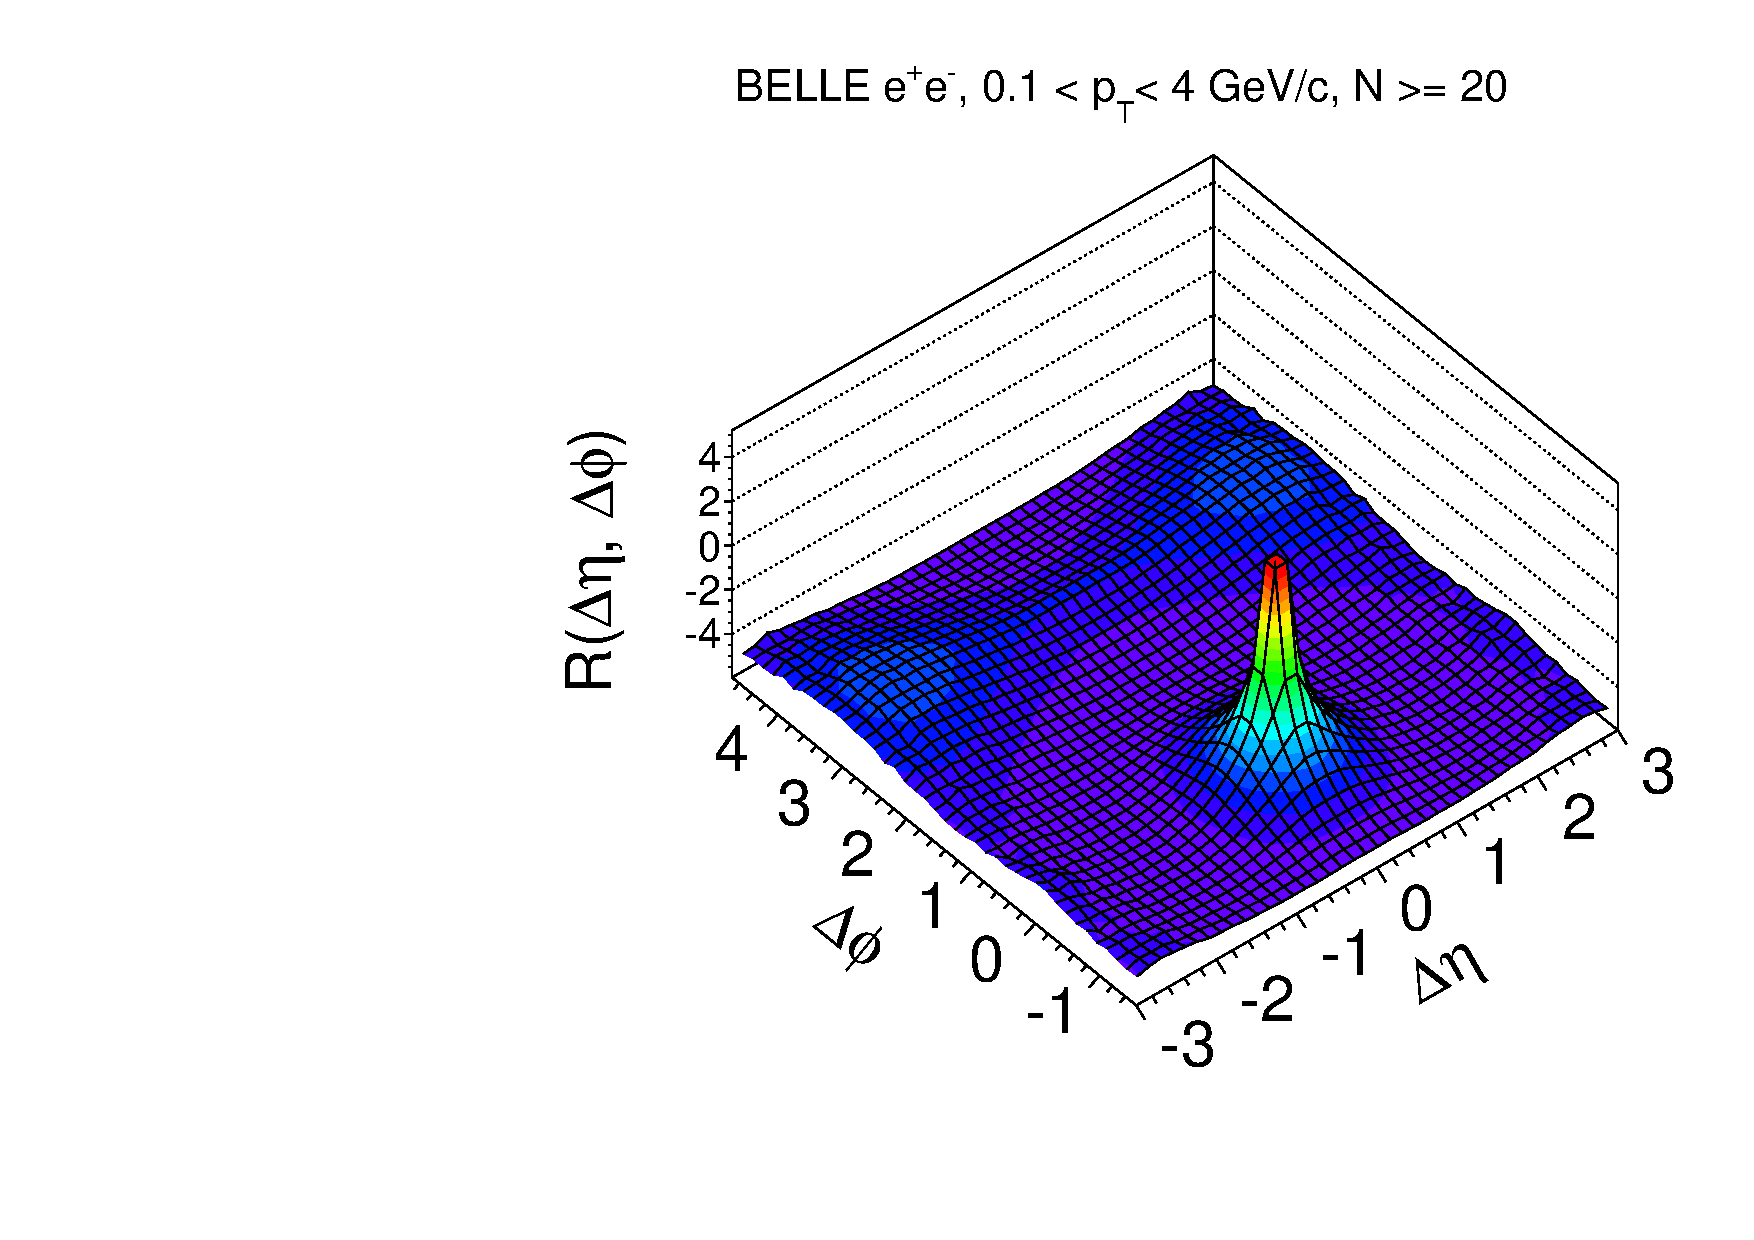
\includegraphics[width=.45\textwidth]{figures/canvasRidgeBelleMult20CutHigh0.pdf}
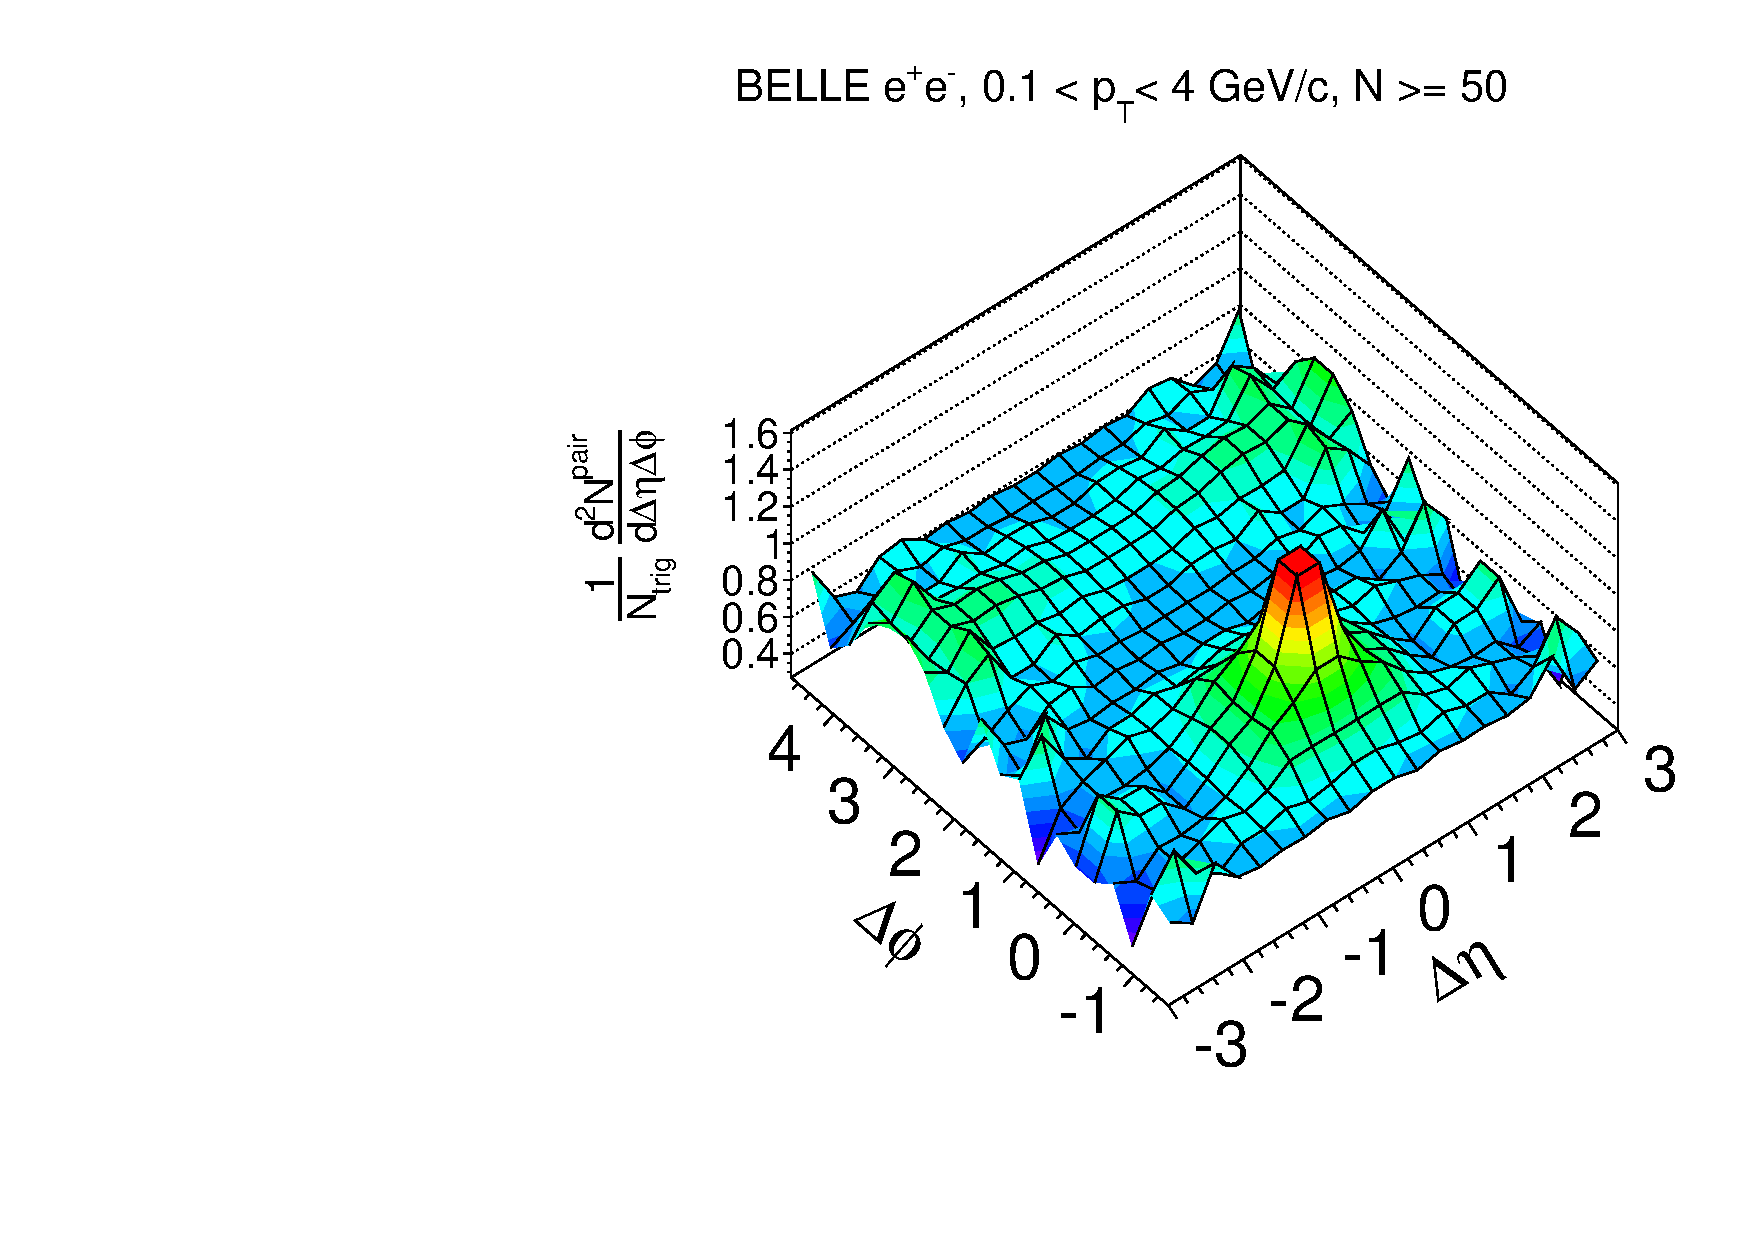
\includegraphics[width=.45\textwidth]{figures/canvasRidgeBelleMult50CutHigh0.pdf}
\caption{Two-particle correlation functions versus $\Delta\eta$ and $\Delta\phi$ in $e^{+}e^{-}$ collisions for events with particle multiplicity $>$ 20 (left) and  $>$ 50 (right).}
\label{fig:ridgeBelle} 
\end{center}
\end{figure}

\begin{figure}[!htb]
\begin{center}
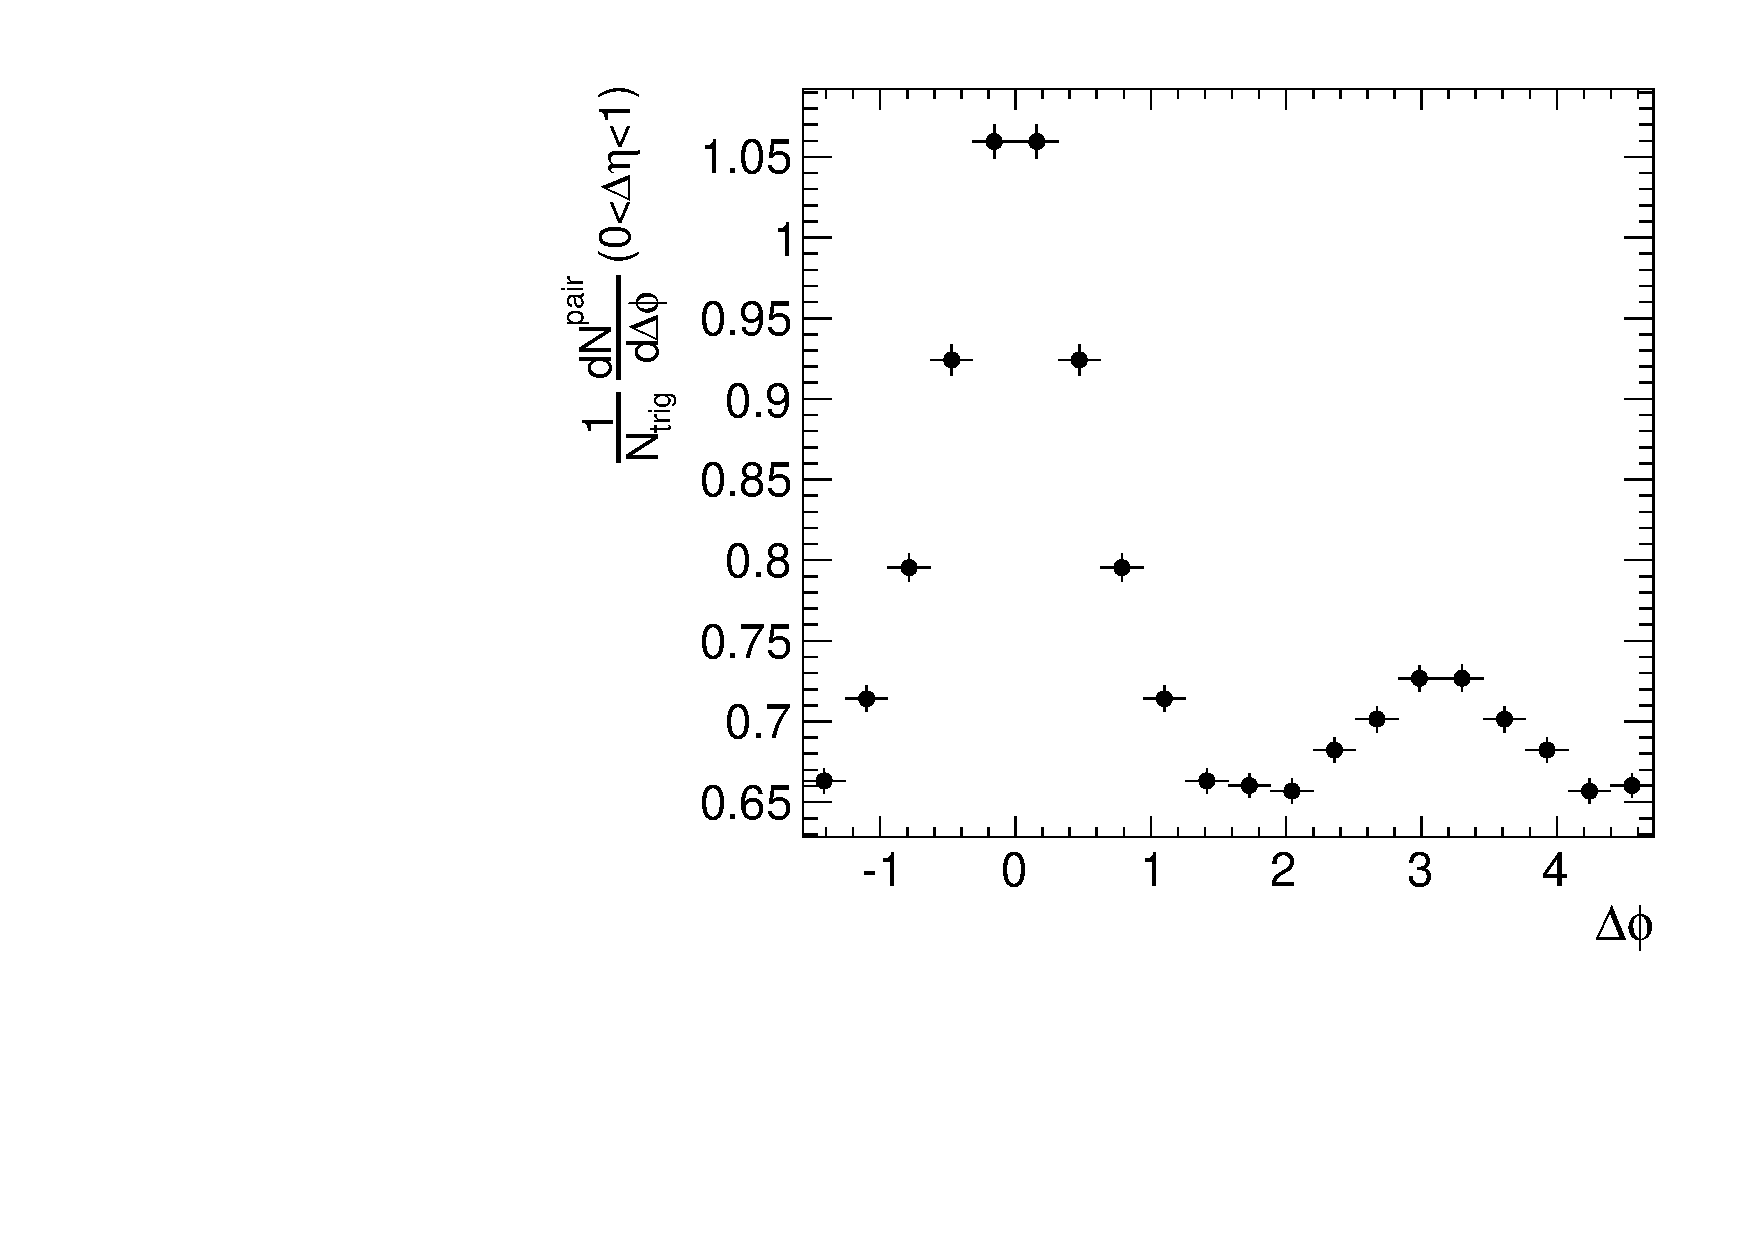
\includegraphics[width=.45\textwidth]{figures/canvasProjection_isBelle1_mult50_eta01.pdf}
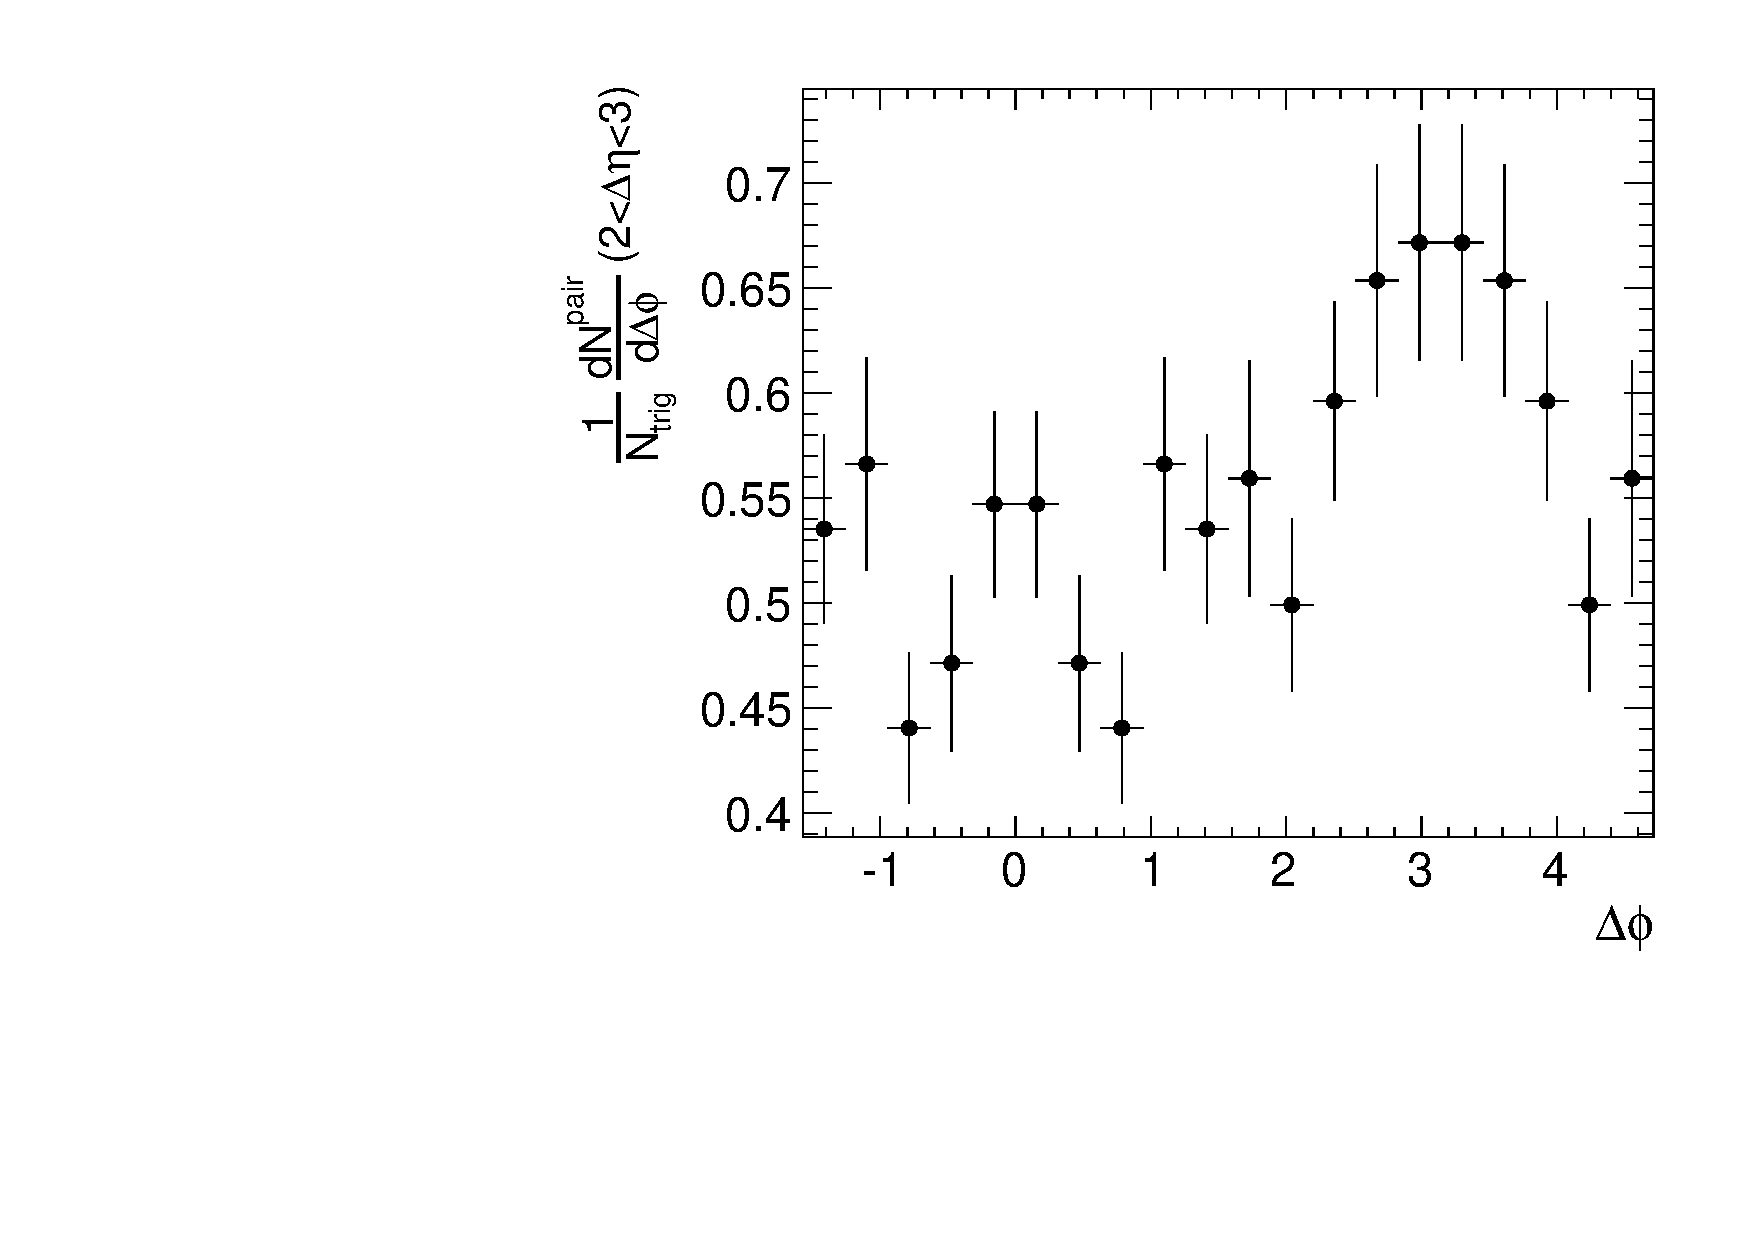
\includegraphics[width=.45\textwidth]{figures/canvasProjection_isBelle1_mult50_eta23.pdf}
\caption{Two-particle correlation functions as a function of  $\Delta\phi$ in $e^{+}e^{-}$ in the pseudorapidity ranges 0$<\Delta \eta<$1 (left) and 2$<\Delta \eta<$3 (right).}
\label{fig:ProjectionMult50} 
\end{center}
\end{figure}

